\documentclass[tikz, margin=5mm]{standalone}
\usepackage[utf8]{inputenc}
\usepackage{xeCJK}
\usetikzlibrary{arrows, positioning}
\usetikzlibrary{calc,shapes.multipart,chains}
\usetikzlibrary{shapes.geometric}
\usetikzlibrary{shapes,snakes}
\usetikzlibrary {arrows.meta}
\usetikzlibrary{fit, backgrounds}
\usepackage{xcolor}
\definecolor{mycolor}{RGB}{84,104,255}
\tikzset{fit margins/.style={/tikz/afit/.cd,#1,
    /tikz/.cd,
    inner xsep=\pgfkeysvalueof{/tikz/afit/left}+\pgfkeysvalueof{/tikz/afit/right},
    inner ysep=\pgfkeysvalueof{/tikz/afit/top}+\pgfkeysvalueof{/tikz/afit/bottom},
    xshift=-\pgfkeysvalueof{/tikz/afit/left}+\pgfkeysvalueof{/tikz/afit/right},
    yshift=-\pgfkeysvalueof{/tikz/afit/bottom}+\pgfkeysvalueof{/tikz/afit/top}},
    afit/.cd,left/.initial=2pt,right/.initial=2pt,bottom/.initial=2pt,top/.initial=2pt}
\begin{document}
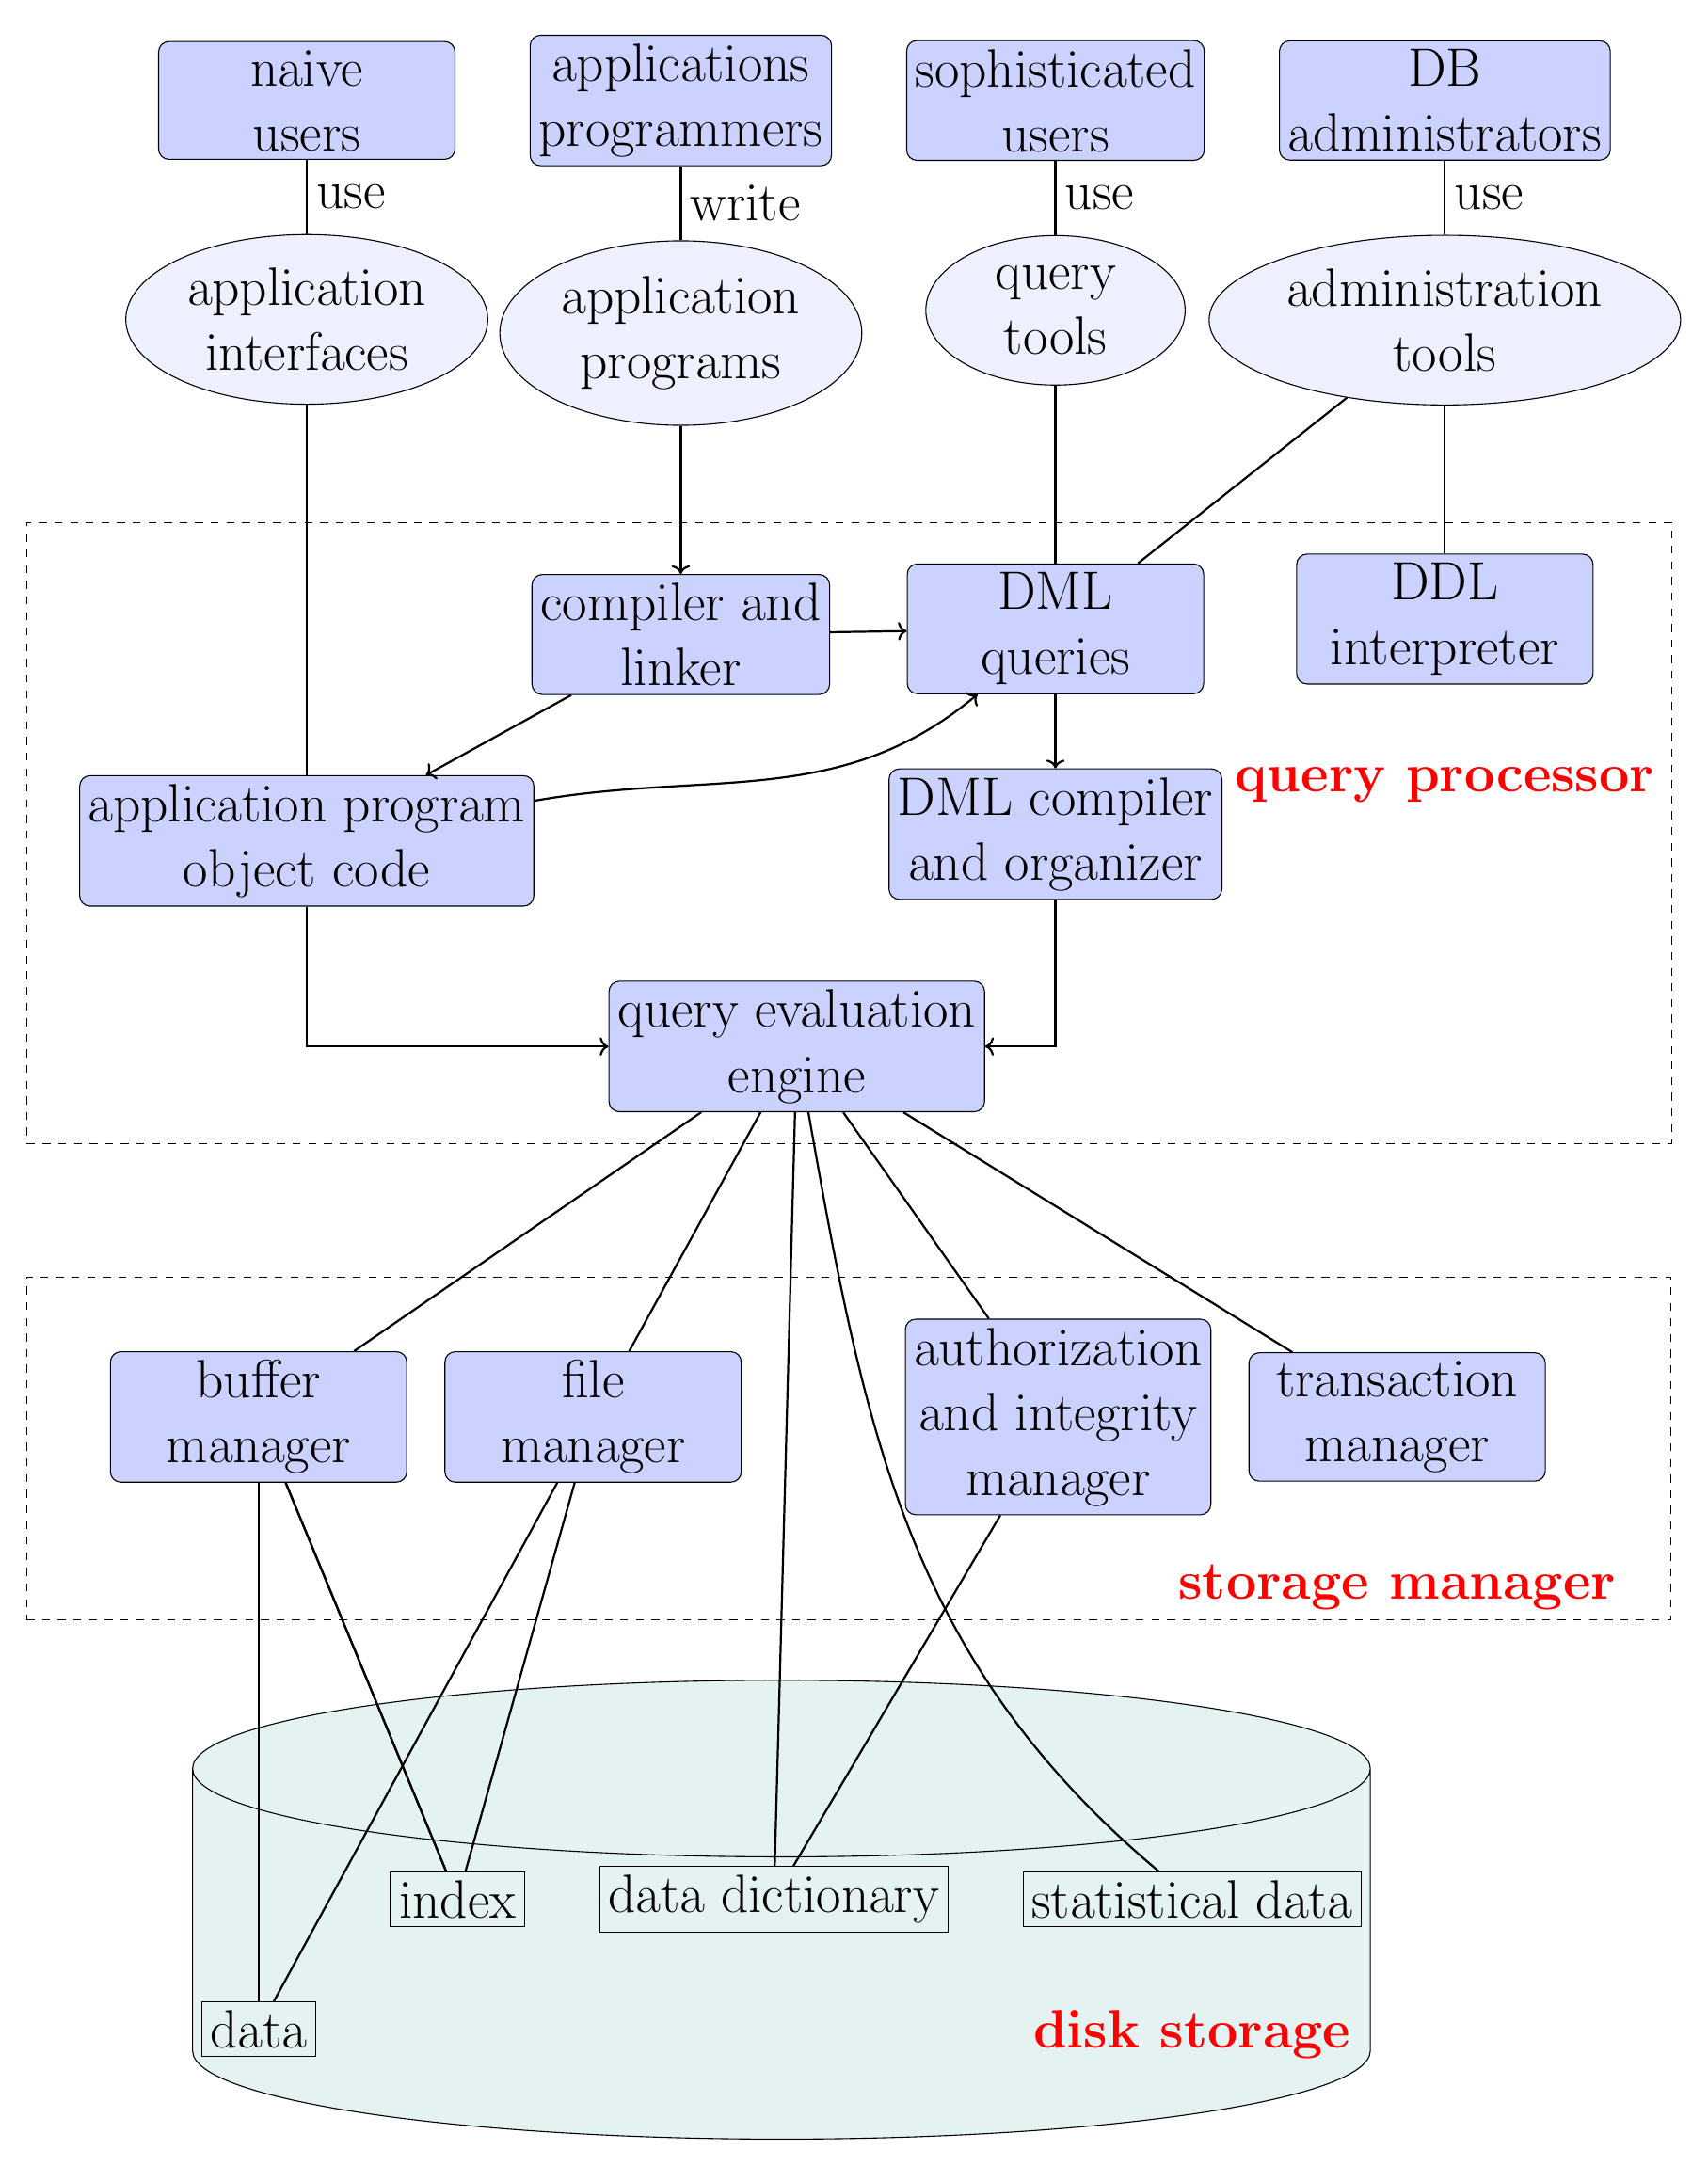
\begin{tikzpicture}[mynode2/.style={fill=mycolor!10, align=center, minimum width=35mm, draw, ellipse, font=\huge}, mynode/.style={fill=mycolor!30, draw, rounded corners, minimum width=40mm, minimum height=10mm, align=center, font=\huge},]
  
    \matrix [column sep=1cm, anchor=center] (users)
    {
      \node[mynode](nuser) {naive \\ users};  & 
      \node[mynode](apppro) {applications \\programmers}; &
      \node[mynode](susers) {sophisticated \\ users}; &
      \node[mynode](dba) {DB \\ administrators}; \\
    };


    \node[mynode2, below=of nuser](appinterface){application \\ interfaces};

    \draw[thick] (nuser) -- node[right]{\huge use} (appinterface);

    \node[mynode2, below=of apppro](apps) {application \\ programs};
    \draw[thick] (apppro) -- node[right]{\huge write} (apps);

    \node[mynode2, below=of susers](querytool) {query \\tools};
    \draw[thick] (susers) -- node[right]{\huge use} (querytool);

    \node[mynode2, below=of dba](dbatool) {administration \\tools};
    \draw[thick] (dba) -- node[right]{\huge use} (dbatool);

    \node[mynode, below=of appinterface, yshift=-4cm](code){application program \\ object code};

    \node[mynode, below=of apps, yshift=-1cm](linker) {compiler and \\linker};

    \draw[<-, thick] (code) -- (linker);


    \node[mynode, below=of querytool, yshift=-1.4cm](dml){DML \\ queries};
    \draw[->, thick] (code) to[in=-140, out=10] (dml);
    \draw[->, thick] (linker) -- (dml);
    \node[mynode, below=of dbatool, yshift=-1cm](ddl){DDL\\ interpreter};

    
    \draw[thick] (querytool) -- (dml);
    \draw[thick] (dbatool) -- (dml);
    \draw[thick] (dbatool) -- (ddl);

    \draw[->, thick] (apps) -- (linker);
    \draw[thick] (appinterface) -- (code);

    \node[mynode, below=of dml] (dmlcompiler){DML compiler \\ and organizer};

    \draw[->, thick] (dml) -- (dmlcompiler);
    
    \node[mynode, below right=of code](engine) {query evaluation\\engine};

    \draw[thick, ->](code)|-(engine);
    \draw[thick, ->] (dmlcompiler) |- (engine);

    \node[below=of ddl, red]{\textbf{\huge{query processor}}};

    \node[fit=(code)(linker)(dml)(ddl)(engine)(dmlcompiler), dashed, draw, fit margins={left=10pt,right=15pt,bottom=6pt,top=6pt}](queryprocessor) {};

    \node[mynode, below=of code, yshift=-5cm, xshift=-.65cm](buffer) {buffer \\ manager};

    \node[mynode, right=of buffer, xshift=-.5cm](file) {file \\manager};

    \node[mynode, right=of file,xshift=1.2cm](integrity){authorization \\and integrity \\ manager};
    \node[mynode, right=of integrity, xshift=-.5cm](transaction){transaction \\manager};

    \node[fit=(buffer)(file)(integrity)(transaction), draw, dashed, fit margins={left=16pt,right=24pt,bottom=20pt,top=8pt}]{};

    \draw[thick] (engine) -- (buffer);
    \draw[thick] (engine) -- (file);
    \draw[thick] (engine) -- (integrity);
    \draw[thick] (engine) -- (transaction);
    
    \node[red, below=of transaction]{\textbf{\huge{storage manager}}};


    \node[draw, below=of buffer, yshift=-6cm,font=\huge](data){data};

    \node[draw, above right=of data, font=\huge](index){index};

    \node[draw, right=of index, font=\huge](dir){data dictionary};

    \node[draw, right=of dir, font=\huge](sta){statistical data};

    \draw[thick] (data) -- (buffer);
    \draw[thick] (data) -- (file);
    \draw[thick] (index) -- (buffer);
    \draw[thick] (index) -- (buffer);
    \draw[thick] (index) -- (file);

    \draw[thick] (integrity) -- (dir);
    \draw[thick] (engine) -- (dir);
    \draw[thick] (engine) to[out=-80,in=140] (sta);



        \begin{scope}[on background layer]
            \node [fit=(data)(index)(dir)(sta),cylinder, shape border rotate=90, draw, aspect=.15,fill=teal!10] {};
        \end{scope}

    \node[below=of sta, red]{\textbf{\huge{disk storage}}};

\end{tikzpicture}
\end{document}